\documentclass{article}
\title{DS-GA-1008 Assignment 1}
\author{LongCat: Catherine Olsson and Long Sha and Kevin Brown}

\usepackage{graphicx}
\usepackage{caption}
\usepackage{subcaption}
\usepackage{amsmath}
\usepackage{enumerate}
\usepackage{natbib}
\usepackage{fullpage}

\begin{document} \maketitle

%Gaussian kernel: Didn't help. Above 0.35, maybe helped?  Dimensionality of
%first two layers (nstates): To 128 (helped) Normalization kernel size: can
%only be run on CPU

\section{Summary of Modifications}

Overall, we tried three significant modifications to the tutorial code
provided:

\begin{enumerate}
\item We added a windowing step in preprocessing, designed to eliminate distracting information (including adjacent house numbers unrelated to the target digit) by obscuring the edges of the images. This modification is described in the Preprocessing section. It ultimately did not improve performance, so in the submitted model we set the width of the window to have no effect, although the ability to decrease the window size is present in the submitted code.

\item We increased the dimensionality of the first two layers, from 64 to 128. This modification is described in the Architecture section. It improved our performance.

\item We tried varying sizes of normalization kernel; however, we were able to try out these modification only on the CPU, not on the GPU, and the tradeoff with speed was not worth it in the last few days before the deadline, so we did not include these modifications in our submitted model.
\end{enumerate}

\section{Preprocessing}

\subsection{Standard preprocessing}
We preprocessed each image in the following manner. First, we converted the
images from RGB representations to YUV, to separate luminance from color, with
the working assumption that pixels that are part of address numbers will have
different luminance, but possibly similar color. (Note: because torch's rgb2yuv
requires floating point representation, we recast the original representation of the data.

Next, we normalized each feature globally, by subtracting the global mean for
each channel, and dividing by the standard deviation (zscore), for the train
data. We then used this mean and standard deviation to transform the test data
(to keep training and testing data separate).

\subsection{Gaussian windowing}
The first feature we attempted to implement was Gaussian windowing in the preprocessing stage. We noticed that in the housenumber dataset, many of the numerals were immediately adjacent to other numerals, as shown in Figure~\ref{fig1}. We were concerned that these adjacent features would be picked up by the algorithm and might contribute to wrong labels. We hypothesized that since we have external prior knowledge that the relevant information is contained within the center of the image, we might improve performance by including our priors, by intentionally obscuring the edges of the image. We included an option to window the input images by a gaussian of a fixed large height and variable width. Figure~\ref{fig1} shows the effect of windowing the image by a Gaussian with standard deviation of $0.25$ the image width. 

We determined, by testing on small-sized test sets, that Gaussian windowing did not noticeably improve performance. Performance remained high at window widths down to approximately $0.35$ and began to decline at narrower widths. Therefore for our final model we did not include a Gaussian window term, although our code retains the ability to include one. We realize that part of the failure to see an effect may be because normalization has undone much of our efforts. We intend to investigate and learn more about the effects of preprocessing and the role of normalization.

\begin{figure}[h]
          \centering
          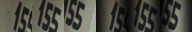
\includegraphics[width=0.8\textwidth]{housenumbers_win.png}
          \caption{Gaussian window preprocessing: Before (left) and after (right)}
          \label{fig1}
\end{figure}

\section{Architecture}

We used the 'convnet' and 'cuda' arguments to the provided code. This produces a model with two stages of convolutional filter-nonlinear-pooling architecture, followed by a standard 2-layer neural network.

The input size is 3 color channels, and 32-by-32 pixels.

We increased the number of filters in the first two layers, to 128 in both cases, which improved performance. We kept the filter size at 5, and the pooling size at 3.

We assume that the number of neurons can be calculated as follows: The input layer contains $32*32*3=3072$ neurons, one per pixel and RGB; Layer One has 128 convolutional filter banks, where each bank convolutionally represents one neuron per input pixel with the same filters/weights shared by each neuron, makes $128 * 32*32 = 131072$ neurons in layer 1; These are then pooled in neighborhoods of size $3*3$ to reduce to $14563 = 113*128$ inputs to the second layer; Layer Two has 128 neurons per 113 of those Layer One stacks, so it has $14563$ neurons itself; finally, there are $128$ neurons in the final layer in the 2-layer neural network at the end. By our calculations this gives rise to \textbf{a total of $3072 + 131072 + 14563 + 128 = 148835$ neurons}. However, as we have not yet learned in class what counts as a ``neuron'' in these networks, we are not certain that we have done this correctly.

\section{Learning Techniques and Training Procedure}
No data augmentations were used beyond the standard preprocessing. We used a dropout probability of 0.5 on the third layer to regularize neurons and prevent `coadaptation'.

We used standard stochastic gradient descent, since the optimization problem is
non-convex for our architecture. We used the default values for the following parameters as provided in the existing code:
\begin{itemize}
\item Learning Rate $1 \times 10^{-7}$
\item Momentum of $0$
\item Loss function: negative log likelihood (nll)
\item Train/validation split: $73257/26032$
\item Training/validation error: So far we have only trained our model based on the training dataset from the assignment, without splitting the training dataset into validation set. Although we certainly did not train our model on the test dataset, nonetheless we did select the model that had the best performance on the test set, so in that sense our results are not fully clean. A fully clean demonstration of the success of an algorithm would require fully held-out data that was never seen by the creators nor used in manually crafting model details, above and beyond never having been by the model in the training step.
\end{itemize}

\end{document}
